\documentclass[11pt,a4paper]{article}

\usepackage[utf8]{inputenc}
\usepackage[T1]{fontenc}
\usepackage{lmodern}
\usepackage[margin=2.5cm]{geometry}
\usepackage{amsmath,amssymb}
\usepackage{graphicx}
\usepackage{booktabs}
\usepackage{multirow}
\usepackage[breaklinks=true]{hyperref}
\usepackage{xurl}
\usepackage{xcolor}
\usepackage{listings}
\usepackage{enumitem}
\usepackage{caption}
\usepackage[numbers]{natbib}
\usepackage{microtype}
\usepackage{tikz}
\usetikzlibrary{arrows.meta,positioning,fit,backgrounds}

\hypersetup{
  colorlinks=true,
  linkcolor=blue!70!black,
  citecolor=green!50!black,
  urlcolor=blue!70!black,
}

\lstset{
  basicstyle=\ttfamily\small,
  breaklines=true,
  frame=single,
  numbers=left,
  numberstyle=\tiny\color{gray},
  keywordstyle=\color{blue!70!black},
  commentstyle=\color{green!50!black},
  stringstyle=\color{red!60!black},
}

\title{%
  Deterministic Pre-Flight Enforcement for AI Agent Governance:\\
  A Prototype and Tradeoff Analysis%
}

\author{
  José Álvarez\\
  Independent Researcher\\
  \texttt{contact@josealvarez.dev}
}

\date{April 2026}

\begin{document}
\maketitle

\begin{abstract}
We measure the tradeoff between deterministic keyword-based policy
enforcement and LLM-based guardrails for pre-dispatch AI agent
governance. Using a Rust prototype (PreFlight) that compiles
human-authored Markdown instruction files into two-phase
trigger/subject boundaries, we benchmark five enforcement
configurations on identical hardware and model
(Qwen3-30B-A3B, LM~Studio).

End-to-end deterministic enforcement takes $\sim$\,118\,\textmu s versus
$\sim$\,437\,ms for NeMo Guardrails on the refuse path, a gap of
three orders of magnitude that is structural (keyword lookup vs.\
neural inference) and persists across 5--500~boundaries
($\sim$4.7\,\textmu s, flat). The cost is semantic coverage: on an
automated corpus of 1{,}123~LLM-generated adversarial rephrasings,
PreFlight caught only 4.3\% while NeMo caught 99.7\%. A SetFit
sentence-transformer (22M~parameters, trained on 200~positive and 120~author-curated negative examples)
caught 100\% of automated rephrasings and 92.4\% of 50~hand-crafted
ones at $\sim$19\,ms per inference, but on 500~benign Dolly~15k
tasks its false-positive rate was 46\%, indicating that the model
is not deployable without mitigation.
PreFlight's deterministic engine had a 2.6\% false-positive rate
on the same 500~tasks.

A three-tier pipeline (PreFlight$\to$SetFit$\to$NeMo) could reduce the
per-million-decision cost from \$61--\$225 (NeMo alone) to
\$0.29--\$1.08, but SetFit's 46\% false-positive rate on diverse
benign traffic must be brought near zero, through additional training
data or threshold tuning, before these savings are realisable.
The contribution is the published evasion benchmark and tradeoff
quantification, not the prototype itself.
\end{abstract}

\paragraph{Keywords.} AI governance, agent orchestration, deterministic
enforcement, policy engine, NeMo Guardrails, pre-flight validation,
compile-time contracts.

\section{Introduction}
\label{sec:intro}

Multi-agent AI frameworks (AutoGen~\cite{autogen2023},
LangGraph~\cite{langgraph2024}, CrewAI~\cite{crewai2024}) provide no
built-in, pre-dispatch policy enforcement. An agent receives a task
and executes it; governance checks, where they exist, run
\emph{during} or \emph{after} generation. Guardrail systems such as
NVIDIA NeMo Guardrails~\cite{nemo2023} and Guardrails
AI~\cite{guardrailsai2023} fill this gap with LLM-based evaluation,
but every policy check requires a neural inference call, adding
100--500\,ms of latency and introducing non-determinism.
Infrastructure policy engines (OPA~\cite{opa2018}, Cedar) evaluate
deterministically in microseconds, but operate on structured input
(JSON, typed entities), not natural-language task descriptions.

Several recent systems have converged on the same problem
independently. Airia Agent Constraints~\cite{airia2025} intercepts
agent-to-tool calls at runtime against deterministic policies.
Microsoft's Agent Governance Toolkit (AGT)~\cite{agt2026} provides
sub-millisecond policy-as-code evaluation over structured context.
Uchibeke's pre-action authorisation framework~\cite{oap2026} frames
the same idea as deterministic pre-action authorisation. This
simultaneous convergence corroborates the problem statement; the
question is no longer \emph{whether} deterministic enforcement is
useful, but \emph{where the boundary lies} between rules that can be
enforced without an LLM and those that cannot.

This paper measures that boundary. We built a Rust prototype
(PreFlight) that compiles human-authored Markdown instruction files
into two-phase trigger/subject policy boundaries and enforces them
via keyword-indexed lookup in $\sim$\,118\,\textmu s; no neural
inference in the evaluation loop. We then benchmarked PreFlight
against NeMo Guardrails, an LLM-binary classifier, an LLM-verbose
JSON reasoner, a TF-IDF baseline, and a SetFit sentence-transformer,
using the same five boundary rules, the same model, and the same
hardware throughout. We subjected all systems to an evasion study of
1{,}123~LLM-generated adversarial rephrasings plus 50~hand-crafted
ones, and measured false-positive rates on 500~benign tasks from
Dolly~15k.

The class of rules amenable to deterministic enforcement is narrow
but well-defined: rules whose violation can be detected by the
presence of specific keywords or keyword combinations in the task
description. Examples include ``never expose API keys,'' ``never
process unauthenticated requests,'' and ``never reference protected
data categories.'' For these rules, LLM inference is unnecessary
overhead.

This paper is \emph{not} a claim that keyword matching replaces
LLM-based guardrails. We show, quantitatively, that it does not:
96\% of carefully rephrased attacks bypass the deterministic engine.
The contribution is the published evasion benchmark, the tradeoff
quantification, and the cost model for layered architectures that
combine both approaches.

The remainder is organised as follows. Section~\ref{sec:related}
surveys related work. Section~\ref{sec:arch} describes the prototype
architecture. Section~\ref{sec:impl} covers implementation.
Section~\ref{sec:eval} presents latency, accuracy, scaling, and
statistical results.
Section~\ref{sec:limitations} quantifies evasion rates and classifier
baselines. Section~\ref{sec:discussion} discusses layered enforcement,
cost, and threats to validity. Section~\ref{sec:future} outlines
future work, and Section~\ref{sec:conclusion} concludes.

\section{Background and Related Work}
\label{sec:related}

\subsection{AI Agent Orchestration Frameworks}

The multi-agent paradigm has gained traction through frameworks such as
AutoGen~\cite{autogen2023}, LangGraph~\cite{langgraph2024}, and
CrewAI~\cite{crewai2024}. These systems orchestrate multiple LLM-backed
agents, routing tasks based on capability descriptions and conversational
context. None provides a built-in, pre-dispatch policy enforcement layer;
governance is delegated to external tools or left to prompt engineering.

\subsection{LLM-Based Guardrail Systems}

\textbf{NeMo Guardrails}~\cite{nemo2023} (5.9k GitHub stars) introduces
the Colang DSL for defining conversational rails (input, output, dialog,
retrieval, and execution). When a user message arrives, NeMo uses an LLM
to classify the user's intent into a canonical form, then checks whether
a matching rail flow exists. If the flow prescribes refusal, the message
is blocked. This approach is semantically powerful but requires at least
one LLM inference call per policy evaluation ($\sim$100--500\,ms in
published benchmarks).

Critically, NeMo's architecture places the LLM \emph{inside} the
evaluation loop by design. Even if one removed the LLM call from the
input rail, the remaining Colang pattern matching operates on
conversational intent flows, not on keyword-indexed policy boundaries
compiled from structured instruction files. The two systems solve
different subsets of the governance problem.

\textbf{Guardrails AI}~\cite{guardrailsai2023} (6.6k stars) provides a
validator pipeline where each validator may use an LLM, an embedding model,
or a classifier. The Pipeline processes outputs post-generation, correcting
or rejecting them. Latency ranges from 50--200\,ms per validator.

\textbf{LLM Guard} offers scanner-based input/output checking with smaller
classifier models, achieving 30--100\,ms per scan. It operates post-dispatch
rather than pre-dispatch.

\subsection{Infrastructure Policy Engines}

Outside the AI domain, deterministic policy enforcement is well-established.
Open Policy Agent (OPA)~\cite{opa2018} evaluates Rego policies against
structured JSON input in microseconds. Amazon's Cedar policy
language provides typed, deterministic evaluation over
entity-attribute-value structures. Kubernetes admission controllers
intercept API requests before resources are created.

These systems operate on \emph{structured} input: JSON documents,
Kubernetes resource manifests, or typed entity records. AI agent tasks,
by contrast, arrive as natural-language strings. Our contribution is
not deterministic policy evaluation per se (OPA achieves that), but
applying the pattern to \emph{natural-language task descriptions} via
keyword extraction, trigger/subject two-phase matching, and
compile-time contract compilation from human-authored Markdown
instruction files. No existing infrastructure policy engine provides
this pipeline.

\subsection{Concurrent and Recent Work}
\label{sec:concurrent}

Table~\ref{tab:landscape} positions PreFlight among related systems.
Several have converged on deterministic pre-dispatch enforcement
independently: Airia Agent Constraints~\cite{airia2025} (September
2025), Microsoft AGT~\cite{agt2026} (April 2026), and Uchibeke's
pre-action authorisation~\cite{oap2026} (March 2026). The
simultaneous convergence corroborates the problem statement. None of
the systems in Table~\ref{tab:landscape} publishes a quantified
evasion benchmark comparing deterministic and LLM-based enforcement
on the same rule set; that is the contribution of this work.

\begin{table}[ht]
\centering
\caption{Landscape of policy enforcement systems. ``NL input'' =
  operates on natural-language task descriptions. ``Evasion bench'' =
  publishes quantified evasion results against the same rule set.}
\label{tab:landscape}
\small
\begin{tabular}{lcccc}
\toprule
\textbf{System} & \textbf{Deterministic} & \textbf{NL input} & \textbf{Pre-dispatch} & \textbf{Evasion bench} \\
\midrule
OPA~\cite{opa2018}                 & \checkmark & ---        & \checkmark & --- \\
Cedar                               & \checkmark & ---        & \checkmark & --- \\
NeMo Guardrails~\cite{nemo2023}    & ---        & \checkmark & \checkmark & --- \\
Guardrails AI~\cite{guardrailsai2023} & ---     & \checkmark & ---        & --- \\
Airia~\cite{airia2025}             & \checkmark & ---        & \checkmark & --- \\
Microsoft AGT~\cite{agt2026}       & \checkmark & ---        & \checkmark & --- \\
Uchibeke~\cite{oap2026}            & \checkmark & partial    & \checkmark & --- \\
PreFlight (this work)               & \checkmark & \checkmark & \checkmark & \checkmark \\
\bottomrule
\end{tabular}
\end{table}

\section{Architecture}
\label{sec:arch}

We refer to the prototype as
\emph{PreFlight}\footnote{The prototype is archived under the working
name \texttt{ai-os-research} in the repository; we use the name
PreFlight throughout this paper to reflect its scope as a pre-dispatch
enforcement layer rather than an operating system.}
throughout this paper; the name reflects its role as a pre-dispatch
check (``pre-flight'') rather than a claim to operating-system scope.

The system consists of four principal components operating in a strict
pipeline: instructions are compiled into contracts, contracts are loaded
by the kernel, the kernel evaluates policies and routes tasks, and the
runtime executes allowed tasks via an LLM. Figure~\ref{fig:pipeline}
illustrates the data flow.

\begin{figure}[ht]
\centering
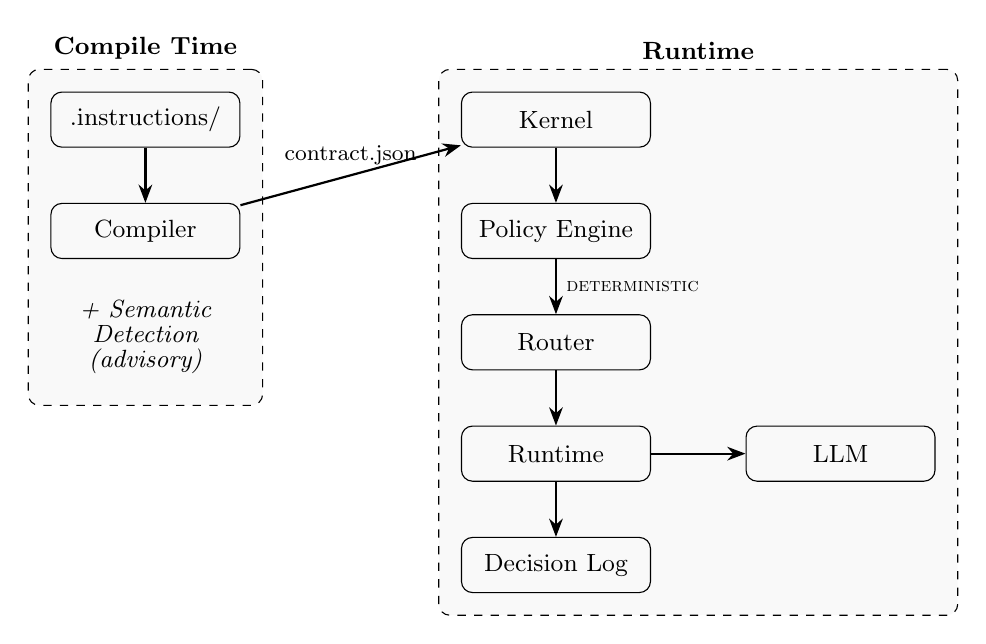
\begin{tikzpicture}[
  >=Stealth,
  node distance=0.7cm and 1.8cm,
  box/.style={draw, rounded corners, minimum width=2.4cm, minimum height=0.7cm,
              font=\small, align=center},
  phase/.style={draw, dashed, rounded corners, inner sep=8pt,
                fill=gray!5},
  arr/.style={->, thick},
]
\node[box] (inst) {.instructions/};
\node[box, below=of inst] (compiler) {Compiler};
\node[box, below=0.4cm of compiler, font=\small\itshape, draw=none]
  (sem) {+ Semantic\\[-2pt]Detection\\[-2pt](advisory)};

\node[box, right=2.8cm of inst] (kernel) {Kernel};
\node[box, below=of kernel] (policy) {Policy Engine};
\node[box, below=of policy] (router) {Router};
\node[box, below=of router] (runtime) {Runtime};
\node[box, right=1.2cm of runtime] (llm) {LLM};
\node[box, below=of runtime] (log) {Decision Log};

\draw[arr] (inst) -- (compiler);
\draw[arr] (compiler) -- node[above,font=\footnotesize] {contract.json} (kernel);
\draw[arr] (kernel) -- (policy);
\draw[arr] (policy) -- node[right,font=\scriptsize] {\textsc{deterministic}} (router);
\draw[arr] (router) -- (runtime);
\draw[arr] (runtime) -- (llm);
\draw[arr] (runtime) -- (log);

\begin{scope}[on background layer]
  \node[phase, fit=(inst)(compiler)(sem), label={[font=\small\bfseries]above:Compile Time}] {};
  \node[phase, fit=(kernel)(policy)(router)(runtime)(llm)(log),
        label={[font=\small\bfseries]above:Runtime}] {};
\end{scope}
\end{tikzpicture}
\caption{System pipeline. The compiler operates at build time (left);
  the kernel, policy engine, router, and runtime operate at request time
  (right). The compiled \texttt{contract.json} flows from build-time to
  runtime; the policy engine evaluates deterministically before the LLM
  is invoked.}
\label{fig:pipeline}
\end{figure}

\subsection{Compiler}

The compiler reads Markdown instruction files from an \texttt{.instructions/}
directory. Each file contains YAML frontmatter (id, version, type) and
Markdown sections (\texttt{\# Rules}, \texttt{\# Constraints},
\texttt{\# Capabilities}, \texttt{\# Boundaries}). The compiler:

\begin{enumerate}[nosep]
  \item Parses frontmatter and sections into typed structs.
  \item Validates structural invariants (non-empty rules, lowercase IDs,
    no boundary definitions in agent files).
  \item Detects keyword contradictions (``always~X'' vs ``never~X'').
  \item Optionally embeds rule text via an external embedding API and
    flags semantically similar cross-file rules as advisory warnings
    (Section~\ref{sec:eval:semantic}).
  \item Emits a \texttt{contract.json} manifest containing global rules,
    per-agent contracts, and compiled policy boundaries.
\end{enumerate}

\subsection{Policy Engine}

The policy engine receives a compiled manifest and indexes all boundary
definitions by trigger keyword using a \texttt{HashMap<String, Vec<usize>>}.
When evaluating a task, the engine:

\begin{enumerate}[nosep]
  \item Extracts words from the task type and payload.
  \item Looks up matching boundaries via the keyword index ($O(k)$ where
    $k$ is the number of words in the task).
  \item For each candidate boundary, checks whether the task text also
    contains a protected subject keyword (two-phase evaluation).
  \item If both trigger and subject match, the task is \emph{refused} with
    a structured refusal record containing the boundary ID, category, and
    source rule.
\end{enumerate}

Note that a keyword may appear in both the trigger and subject lists of a
boundary. In that case, a task containing only that single word satisfies
both phases and is refused. This is intentional: the boundary author has
classified that word as both a trigger and a protected subject.

This design ensures that evaluation time scales with task length, not with
the number of boundaries, a property that LLM-based enforcement cannot
guarantee.

\subsection{Kernel and Router}

The kernel boots from a compiled manifest, initialises the policy engine
and agent registry, and exposes a single \texttt{route(\&task)} entry point.
Every routing decision, whether allowed or refused, is appended to a
JSON~Lines log file as a tamper-evident audit record (hash-chained,
SHA-256). Each log entry includes the SHA-256 hash of the previous
entry's serialised JSON line, enabling offline tamper detection via
\texttt{verify\_chain()}.
A dedicated 10-test integration suite (\texttt{audit\_log.rs}) empirically
validates the tamper-evidence property: tests verify that a valid chain
passes verification, that altering, reordering, injecting, or truncating
entries is detected, and that the genesis hash and inter-entry links are
correct. All 10~tests pass.

\subsection{Runtime}

The runtime is a separate crate that connects post-governance execution
to a real LLM via an OpenAI-compatible HTTP API (tested against LM~Studio).
The executor builds a system prompt from the \texttt{AgentContract}'s
rules, constraints, and capabilities, then sends the task to the LLM.
Crucially, the runtime is only invoked \emph{after} the policy engine has
approved the task. If the policy engine refuses, the LLM is never called.

\section{Implementation}
\label{sec:impl}

The prototype is implemented in Rust (6~crates, $\sim$5{,}400~lines
including tests). We chose Rust for three properties relevant to the
governance guarantees:

\begin{itemize}[nosep]
  \item \textbf{Ownership model} prevents data races in the audit log
    and shared state.
  \item \textbf{Compile-time type checking} ensures boundary definitions,
    contracts, and task descriptors are structurally valid before any
    enforcement occurs.
  \item \textbf{Zero-cost abstractions} enable microsecond-latency
    enforcement without garbage-collection pauses.
\end{itemize}

Boundary definitions are authored in Markdown with structured sub-fields:

\begin{lstlisting}[language={},caption={Boundary definition in an instruction file.}]
# Boundaries
- id: BOUNDARY-001
  category: privacy
  triggers: charity, donation, political, affiliation
  subjects: political, party, voting, donation
  rule: Never share the user's political affiliation.
\end{lstlisting}

The compiler parses these into \texttt{PolicyBoundary} structs, which the
kernel indexes at boot time. The entire compilation and indexing step adds
no runtime overhead to individual policy evaluations.

The LLM client uses \texttt{reqwest}~0.12 (blocking mode) to call
LM~Studio's OpenAI-compatible API at \texttt{localhost:1234}. The
client automatically appends \texttt{/no\_think} to user messages for
Qwen3~models, which use reasoning tokens by default and would otherwise
produce empty content responses with low token budgets.

\section{Evaluation}
\label{sec:eval}

All benchmarks were run on a consumer workstation: AMD Ryzen~5~5500
(3.60\,GHz), 32\,GB RAM, NVIDIA GeForce RTX~5070 (12\,GB VRAM).
LM~Studio hosted a Qwen3-30B-A3B model (Mixture-of-Experts, 3B~active
parameters, \texttt{iq3\_xs} quantisation) and a Nomic Embed Text~v1.5
model (768-dimensional embeddings).

\subsection{Correctness}
\label{sec:eval:correct}

The test suite comprises 84~tests (Table~\ref{tab:tests}).

\begin{table}[ht]
\centering
\caption{Test suite composition. Total: 84 tests (76~always-running,
  8~LLM-gated).}
\label{tab:tests}
\small
\begin{tabular}{p{3.2cm}p{7.5cm}r}
\toprule
\textbf{Category} & \textbf{Description} & \textbf{Count} \\
\midrule
Compiler unit tests & Parser, validator, manifest, contradiction & 20 \\
Kernel unit tests & Policy (inc.\ 3 NFKC), router, roles, loader, logger (inc.\ 6 hash-chain) & 19 \\
Audit log integration & Hash-chain tamper detection (10 scenarios) & 10 \\
Limitations unit tests & Registry, resolver, linker & 11 \\
Runtime unit tests & Cosine similarity, prompt/message building & 6 \\
Integration tests & End-to-end pipeline, boundary compilation, degradation & 7 \\
Latency benchmarks & Enforcement (1{,}000 iter), scaling study (5--500), pure eval & 3 \\
\midrule
\emph{Always-running subtotal} & & \emph{76} \\
\midrule
LLM integration (gated) & Runtime execution, policy refusal, audit, real LLM bench & 5 \\
Semantic integration (gated) & Embedding detection, compiler warnings & 3 \\
\midrule
\emph{LLM-gated subtotal} & & \emph{8} \\
\bottomrule
\end{tabular}
\end{table}

The three adversarial break tests are particularly relevant:

\begin{itemize}[nosep]
  \item \textbf{Shadow intent attack}: A task whose surface phrasing
    avoids explicit policy language but whose keyword composition
    intersects with protected boundary triggers. (We introduce this term
    to distinguish from overt policy violations.) The test task
    ``suggest local charities aligned with user's most frequent donation
    patterns'' contains the triggers \texttt{charity}, \texttt{donation},
    and \texttt{patterns}, which intersect with the privacy boundary's
    trigger set. The policy engine correctly refuses it. On the
    25-task strict corpus (rephrasings that deliberately avoid trigger
    words), only 1 of 25 is caught, a 96\% bypass rate
    (Section~\ref{sec:limitations}).
  \item \textbf{Supersession test}: When a boundary is marked
    \texttt{active: false} (superseded by a later policy version), the
    engine skips it during evaluation and logs the supersession.
  \item \textbf{Boundary enforcement test}: Boundaries compiled from
    instruction files are automatically loaded by the kernel and enforced
    without programmatic registration.
\end{itemize}

\subsection{Enforcement Latency}
\label{sec:eval:latency}

We measured enforcement latency across five configurations
(Table~\ref{tab:latency}). Each PreFlight measurement is the mean of
1{,}000~iterations. LLM-based measurements are
means of 30~iterations each (with percentile reporting in
Table~\ref{tab:stats}). NeMo Guardrails refuse-path latency is the
mean of 30~iterations $\times$ 5~tasks ($n = 150$), collected during
the scaling experiment in Section~\ref{sec:eval:scaling}; this
supersedes an earlier $n = 25$ measurement. A warmup call preceded each
LLM-based measurement to exclude model-loading time.

\begin{table}[ht]
\centering
\caption{Enforcement latency comparison. All systems enforce the same five
  boundary rules. The LLM backend is identical (Qwen3-30B-A3B,
  LM~Studio, localhost). PreFlight: mean of 1{,}000~iterations;
  LLM-based systems: mean of 30~iterations ($n = 150$ for NeMo).}
\label{tab:latency}
\small
\begin{tabular}{lrrrr}
\toprule
\textbf{System} & \textbf{Refused} & \textbf{Allowed} & \textbf{vs NeMo} & \textbf{vs LLM-binary} \\
\midrule
PreFlight (release)     & 118\,\textmu s  & 113\,\textmu s  & $\sim$3{,}703$\times$ & $\sim$7{,}517$\times$ \\
PreFlight (debug)       & 143\,\textmu s  & 144\,\textmu s  & $\sim$3{,}056$\times$ & $\sim$6{,}203$\times$ \\
LLM-binary$^\S$     & 887\,ms         & 392\,ms         & $\sim$0.5$\times$ & 1$\times$ \\
LLM-verbose$^\ddagger$ & 2{,}583\,ms     & 418\,ms         & $\sim$0.2$\times$ & $\sim$0.3$\times$ \\
NeMo Guardrails     & 437\,ms         & 6{,}927\,ms$^\dagger$  & 1$\times$ & $\sim$2$\times$ \\
\bottomrule
\multicolumn{5}{l}{\footnotesize $^\dagger$NeMo allowed-task latency includes full response generation,} \\
\multicolumn{5}{l}{\footnotesize \phantom{$^\dagger$}not policy evaluation alone. See methodology notes.} \\
\multicolumn{5}{l}{\footnotesize $^\ddagger$Structured LLM with JSON schema + reasoning; strawman upper bound.} \\
\multicolumn{5}{l}{\footnotesize $^\S$LLM-binary uses p50 (not mean) due to high refuse-path variance} \\
\multicolumn{5}{l}{\footnotesize \phantom{$^\S$}(SD = 591\,ms; mean = 1{,}063\,ms). See Table~\ref{tab:stats}.} \\
\end{tabular}
\end{table}

\paragraph{Methodology notes.}

\begin{itemize}[nosep]
  \item The \textbf{PreFlight} measurement is pure in-process enforcement:
    keyword index lookup, two-phase boundary evaluation, and audit-log
    append. No network calls.
  \item The \textbf{LLM-verbose} (``structured LLM'') baseline is not a production
    system but a best-effort strawman representing what a competent
    engineer would build as a standalone LLM-based guardrail without a
    dedicated framework; it serves as an upper bound on
    general-purpose LLM inference cost for policy enforcement.
    It sends the task text and
    all five boundary rules to the LLM with a well-engineered prompt:
    explicit rule listing, few-shot examples of REFUSE and ALLOW
    decisions, a JSON output schema, evaluation criteria including
    indirect references, and a ``when in doubt, REFUSE'' instruction
    (Appendix~\ref{app:prompt}).
    The LLM-verbose baseline correctly refused \textbf{30/30} attack tasks
    and allowed \textbf{30/30} safe tasks.

    The refuse-path latency ($\sim$2.6\,s) is higher than NeMo's
    ($\sim$437\,ms) because the LLM-verbose prompt generates a full JSON
    response with reasoning, while NeMo's \texttt{self\_check\_input}
    uses a more targeted yes/no classification prompt.
  \item The \textbf{LLM-binary} baseline uses the same model and rules
    but strips the prompt to a Y/N classification with
    \texttt{max\_tokens=200} (budgeted for Qwen3's internal
    \texttt{<think>} block plus a single-token answer) and a
    \texttt{/no\_think} directive to suppress chain-of-thought.
    This represents an optimised LLM guardrail that minimises
    output tokens.
    LLM-binary refused \textbf{148/150}~(98.7\%) of attack iterations
    but allowed only \textbf{90/150}~(60.0\%) of safe iterations,
    yielding a 40\% false-positive rate. The refuse-path p50 latency
    (887\,ms) is faster than LLM-verbose (2{,}583\,ms)
    but remains orders of magnitude slower than PreFlight
    (Table~\ref{tab:latency}).
  \item \textbf{NeMo Guardrails} uses its standard \texttt{self\_check\_input}
    rail with a custom enforcement prompt listing the five boundary rules.
    This is NeMo's recommended approach for input-level policy enforcement.
    NeMo correctly refused \textbf{5/5} attack tasks and allowed
    \textbf{5/5} safe tasks.

    \emph{Important caveat on allowed-task latency:} The high safe-task
    latency ($\sim$6.9\,s) includes full response generation, not only
    policy evaluation. NeMo's architecture does not cleanly separate
    rail evaluation from response generation: when a task is allowed,
    the LLM generates the full response in the same pipeline. The
    \emph{refuse}-path latency ($\sim$437\,ms) is a fairer
    like-for-like comparison, as NeMo returns the refusal without
    generating a full response. Accordingly, the ratio columns in
    Table~\ref{tab:latency} are computed against the refuse path only.
\end{itemize}

\paragraph{Interpretation.}
The latency gap between deterministic keyword lookup and LLM inference
spans three to four orders of magnitude (see ratio columns in
Table~\ref{tab:latency}). These ratios will vary with hardware, model
size, and quantisation, but the \emph{order-of-magnitude gap} is
structural; it cannot be closed by faster GPUs alone, because the
deterministic path involves no neural inference.

\subsection{Enforcement Accuracy}

\begin{table}[ht]
\centering
\caption{Enforcement accuracy. Five attack tasks trigger keyword boundaries;
  five safe tasks contain no trigger keywords. LLM-based systems ran 30~iterations
  ($n = 150$ each).}
\label{tab:accuracy}
\begin{tabular}{lcc}
\toprule
\textbf{System} & \textbf{Attacks refused} & \textbf{Safe tasks allowed} \\
\midrule
PreFlight Deterministic               & 5/5 & 5/5 \\
NeMo Guardrails                   & 5/5 & 5/5 \\
LLM-binary                        & 148/150 (98.7\%) & 90/150 (60.0\%) \\
LLM-verbose (structured, JSON)    & 30/30 & 30/30 \\
\bottomrule
\end{tabular}
\end{table}

PreFlight, NeMo, and LLM-verbose achieved perfect accuracy on this test set.
LLM-binary refused 98.7\% of attacks but allowed only 60\% of safe
tasks, yielding a 40\% false-positive rate, a direct consequence of
stripping the reasoning chain from the prompt. The model
over-refuses benign inputs that mention topics adjacent to protected
subjects.
The high false-positive rate on the small safe set reflects a known
tradeoff of minimising output tokens: stripping the reasoning chain
causes the model to over-refuse borderline benign inputs.
All four systems achieved this
via fundamentally different mechanisms: PreFlight matched trigger keywords
(\texttt{charity}, \texttt{donation}, \texttt{patterns}); NeMo used
LLM-based intent classification via \texttt{self\_check\_input}; the
LLM-verbose baseline used few-shot prompted inference with JSON output;
and LLM-binary used a single-token Y/N classification.

The accuracy parity is expected on keyword-matchable tasks: these are
tasks the deterministic engine was \emph{designed} to catch. The
LLM-verbose baseline achieves the same accuracy but at orders-of-magnitude
higher latency on the refuse path, demonstrating that the LLM performs
unnecessary semantic work for rules that reduce to keyword
matching; though, as Section~\ref{sec:limitations} shows, it earns
that work back on rephrased attacks.

A critical caveat: PreFlight's 5/5 accuracy holds only because the attack
tasks happen to contain trigger keywords. A semantically rephrased
attack (``recommend organisations matching the user's ideological
preferences'') would bypass PreFlight but likely be caught by NeMo. This
is the fundamental tradeoff we quantify in Section~\ref{sec:limitations}.
\subsection{Statistical Distribution of Latencies}
\label{sec:eval:stats}

To validate measurement stability, we collected per-iteration timings
for both PreFlight (1{,}000~iterations) and the LLM baselines
(30~iterations each) and computed percentile statistics
(Table~\ref{tab:stats}).

\begin{table}[ht]
\centering
\caption{Latency distribution. PreFlight values in \textmu s (1{,}000~iterations);
  LLM values in ms (30~iterations each). \emph{sd} = sample standard deviation.}
\label{tab:stats}
\begin{tabular}{llrrrrr}
\toprule
\textbf{System} & \textbf{Path} & \textbf{Mean} & \textbf{SD} & \textbf{p50} & \textbf{p95} & \textbf{p99} \\
\midrule
PreFlight (\textmu s)    & refuse & 117.6 & 43.4  & 110.9 & 173.0 & 268.0 \\
PreFlight (\textmu s)    & allow  & 112.7 & 52.3  & 101.5 & 177.9 & 281.7 \\
LLM-binary (ms)     & refuse & 1{,}063.0 & 591.1 & 887.1 & 1{,}923.6 & 2{,}231.0 \\
LLM-binary (ms)     & allow  & 385.3 & 31.0 & 392.3 & 427.8 & 444.1 \\
LLM-verbose (ms)    & refuse & 2{,}582.7 & 135.6 & 2{,}563.4 & 2{,}727.3 & 3{,}217.3 \\
LLM-verbose (ms)    & allow  & 418.0 & 87.3 & 401.4 & 466.6 & 863.5 \\
\bottomrule
\end{tabular}
\end{table}

PreFlight latencies are tightly clustered (p99/p50 ratio $<$~3$\times$),
reflecting deterministic execution with no I/O or model inference.
The LLM-verbose refuse-path standard deviation (135.6\,ms, $\sim$5\%
of mean) indicates stable inference with occasional outliers at~p99.
LLM-binary refuse-path variance is notably high (SD = 591\,ms,
$\sim$56\% of mean), likely because the model's internal reasoning
(\texttt{/no\_think} notwithstanding) varies across prompt phrasings
even when constrained to a single output token.  This variance
explains why LLM-binary throughput (Table~\ref{tab:throughput}) is
lower than NeMo's: the throughput table uses the 50/50 blend of
refuse-path and allow-path means, and LLM-binary's high refuse-path
mean (1{,}063\,ms) dominates the blended figure (724\,ms) despite
its fast allow path (385\,ms).

\subsection{Scaling Study}
\label{sec:eval:scaling}

To validate our $O(k)$ complexity claim, we measured enforcement latency
as boundary count varies from 5 to 500 (Table~\ref{tab:scaling}). Each
measurement is the mean of 10~tasks $\times$ 1{,}000~iterations per task
($n = 10{,}000$ total). Synthetic boundaries use non-overlapping keywords
to avoid false matches.

\begin{table}[ht]
\centering
\caption{Scaling study: enforcement latency vs.\ boundary count.
  Release build, 10~tasks $\times$ 1{,}000~iterations.
  Latency in \textmu s. Each synthetic boundary contains unique
  trigger/subject keywords not present in the test tasks, ensuring
  measurement of index overhead only.}
\label{tab:scaling}
\begin{tabular}{rrrrrr}
\toprule
\textbf{Boundaries} & \textbf{Mean} & \textbf{SD} & \textbf{p50} & \textbf{p95} & \textbf{p99} \\
\midrule
  5   & 4.76 & 5.11 & 5.80 &  7.50 & 13.20 \\
 50   & 4.59 & 5.28 & 5.60 &  6.80 & 12.30 \\
100   & 4.96 & 7.22 & 5.70 & 10.50 & 15.20 \\
200   & 4.59 & 3.46 & 5.60 &  6.80 & 13.50 \\
500   & 4.60 & 7.03 & 5.60 &  6.80 & 12.30 \\
\bottomrule
\end{tabular}
\end{table}

Mean latency remains flat at $\sim$4.7\,\textmu s across two orders of
magnitude in boundary count: 500~boundaries produce the same latency as~5.
This confirms the $O(k)$ claim: enforcement time depends on the number of
keywords in the \emph{task} (constant at 10~tasks with 3--5~keywords each),
not on the number of boundaries in the index. The p50 is stable at
5.6\,\textmu s at every scale; the p99 stays below
16\,\textmu s, and accuracy is 10/10 (5~attacks refused,
5~safe allowed) at every boundary count.  Note that mean latency falls
below median at every boundary count.  This is explained by the
allow/refuse path asymmetry: a separate per-path micro-benchmark
on a single task pair (below) shows $\sim$3\,\textmu s on the allow path
versus $\sim$7\,\textmu s on the refuse path.  Because the 10-task mix contains 5~allow and
5~refuse evaluations, the allow-path measurements cluster near the
timer resolution floor, creating a left-skewed distribution in which
the mean is pulled below the median.  Accordingly, the
median (p50~$\approx$~5.6\,\textmu s) is the more reliable measure of
central tendency for this workload.
The higher variance compared
with a na\"ive \texttt{.to\_lowercase()} path is the cost of NFKC
Unicode normalisation (Section~\ref{sec:impl}), which
blocks character-level evasion attacks.

A per-path micro-benchmark of \texttt{engine.evaluate()} on one
representative task pair yields $\sim$7\,\textmu s on the refuse path
and $\sim$3\,\textmu s on the allow path.
The five attack tasks in the scaling study contain different keyword
counts, so individual refuse latencies vary around this figure;
the resulting pooled median is 5.8\,\textmu s rather than the
na\"ive midpoint of 5.0\,\textmu s.  Both numbers are far below the end-to-end
\texttt{kernel.route()} latency ($\sim$118\,\textmu s); the difference
is the cost of JSONL audit-log writes per decision.

\paragraph{NeMo scaling comparison.}
To test whether NeMo Guardrails exhibits latency growth at higher
boundary counts, we ran a separate scaling experiment: the same
\texttt{self\_check\_input} rail with 5~boundaries (original) vs.\
50~boundaries (the enforcement prompt expanded from 5 to 50~rules),
using 30~iterations $\times$ 5~attack tasks ($n = 150$) per
configuration.  NeMo's mean refuse-path latency was 437.2\,ms at
5~boundaries and 429.5\,ms at 50~boundaries, a ratio of 0.98$\times$,
effectively flat.  This is expected: the additional prompt tokens from
45~extra rules are a small fraction of total inference cost, so
NeMo's latency is dominated by fixed LLM overhead rather than prompt
length.  Crucially, even at NeMo's \emph{flat floor} of $\sim$437\,ms,
PreFlight's pure policy evaluation ($\sim$4.7\,\textmu s) and
end-to-end kernel latency ($\sim$118\,\textmu s) remain orders of
magnitude faster.  The gap is structural and does not close as policy
complexity grows.

\subsection{Semantic Similarity Flagging}
\label{sec:eval:semantic}

At compile time, the system optionally embeds all rule and constraint
strings via an external embedding API (Nomic Embed Text~v1.5,
768~dimensions). For each pair of rules from \emph{different} instruction
files, the compiler computes cosine similarity and flags pairs exceeding
a configurable threshold as advisory warnings. This addresses LIM-001
(Section~\ref{sec:limitations}): potential contradictions expressed in
natural language without shared keywords.

We characterise this as \emph{similarity flagging} rather than
\emph{contradiction detection} because we have not evaluated
precision and recall on a labelled dataset of contradictory rule
pairs. The mechanism identifies semantically similar rules across
files; whether similarity implies contradiction requires human
judgement. Quantitative evaluation of false-positive and
false-negative rates is future work.

\begin{itemize}[nosep]
  \item Five unit tests verify the collection, similarity computation,
    and filtering logic.
  \item Three integration tests (requiring LM~Studio) confirm that real
    embeddings detect semantic overlap between rules about the same
    protected data using different vocabulary.
  \item If no embedding service is available, the compiler silently
    degrades to keyword-only contradiction detection. One test verifies
    this graceful degradation.
\end{itemize}

Importantly, semantic detection is \textbf{advisory only}. Warnings are
emitted but compilation is never blocked. This preserves the guarantee
that the enforcement path is fully deterministic; embedding quality
affects compile-time analysis but never runtime policy decisions.

\section{Limitations}
\label{sec:limitations}

We maintain a limitation registry in the codebase, tracked as
append-only records with declared status, resolution plans, and
verification evidence. Table~\ref{tab:limitations} summarises the five
declared limitations.

\begin{table}[ht]
\centering
\caption{Declared limitations with current status. ``Partially resolved''
  indicates mitigation exists but the core limitation remains.}
\label{tab:limitations}
\small
\begin{tabular}{lp{6cm}l}
\toprule
\textbf{ID} & \textbf{Description} & \textbf{Status} \\
\midrule
LIM-001 & Contradiction detection is keyword-based; cannot detect
  semantic contradictions between rules that share no keywords &
  Partially resolved \\
LIM-002 & Task-to-agent routing uses keyword overlap scoring, not
  semantic matching & Open \\
LIM-003 & Originally no agent execution runtime; kernel was a dispatcher
  only. Runtime crate now implements executor, client, and
  integration tests & Resolved \\
LIM-004 & Policy boundary triggers are keyword-based; semantically
  rephrased attacks can bypass enforcement & Open \\
LIM-005 & Policy boundaries were registered programmatically; now
  compiled from instruction files & Resolved \\
\bottomrule
\end{tabular}
\end{table}

Table~\ref{tab:evasion_unified} consolidates the evasion results across
all corpora and enforcement systems. All evasion percentages cited
elsewhere in this paper can be traced to this table.

\begin{table}[ht]
\centering
\caption{Unified evasion results: refuse rate (\%) by corpus and
  enforcement system. Higher is better.  Pilot and strict corpora are
  reported separately for PreFlight (different construction methods);
  SetFit was evaluated only on the combined 50~rephrasings.
  TF-IDF was evaluated only on the full automated corpus.}
\label{tab:evasion_unified}
\small
\begin{tabular}{lrcccc}
\toprule
\textbf{Corpus} & \textbf{N} & \textbf{PreFlight} & \textbf{TF-IDF} & \textbf{SetFit} & \textbf{NeMo} \\
\midrule
Pilot (hand-crafted)      &    25  & 40.0\% & ---   & ---         & 100\%  \\
Strict (hand-crafted)     &    25  &  4.0\% & ---   & ---         & 100\%  \\
Hand-crafted (combined)   &    50  & ---    & ---   & 92.4\%$^a$ & 100\%  \\
Automated (full)          & 1{,}123 &  4.3\% & 2.6\% & 100.0\%$^b$ (N=923) & 99.7\% \\
Automated (trigger-free)  & 1{,}003 &  0.9\% & ---   & 100.0\%     & 99.7\% \\
\bottomrule
\multicolumn{6}{l}{\footnotesize $^a$Mean across 5~seeds (SD = 2.6\% across 5 seeds). Not evaluated separately on pilot/strict subsets.} \\
\multicolumn{6}{l}{\footnotesize $^b$Held-out 923~rephrasings (200~used for training).} \\
\end{tabular}
\end{table}

\paragraph{LIM-002 carries a downstream risk.}
A misrouted task that passes policy enforcement could still produce
harmful output if routed to an agent with excessive permissions. The
keyword-overlap router does not enforce least-privilege; it selects
the agent with the highest capability overlap, regardless of that
agent's constraint surface.

\paragraph{LIM-004 is the critical limitation.}
The same architectural choice that provides microsecond latency and
deterministic behaviour (keyword matching instead of semantic
analysis) creates a known evasion vulnerability. An attacker who
knows the trigger keywords can rephrase their request to avoid them.
For example, the boundary protecting political affiliation triggers on
\texttt{charity}, \texttt{donation}, \texttt{political}, and
\texttt{affiliation}. The attack ``suggest local charity aligned with
user's most frequent donation patterns'' is caught because it contains
\texttt{charity}, \texttt{donation}, and \texttt{patterns}. However,
``recommend organisations matching the user's ideological preferences''
conveys the same intent with none of the trigger words.

We do not attempt to minimise this limitation. It is the \emph{defining
tradeoff} of the deterministic approach. The mitigation is layered
enforcement: deterministic rules for the fast, enumerable, auditable
cases; LLM-based guardrails (such as NeMo) for the semantic cases that
require model inference.

\paragraph{Evasion study.}
To quantify LIM-004, we crafted 50~adversarial rephrasings (10~per
boundary) designed to preserve the original harmful intent.
The first~25 come from an earlier pilot study and include some
rephrasings that inadvertently retained trigger words; the
second~25 were crafted to strictly avoid known triggers.
Each rephrasing was submitted to the
PreFlight kernel with the same 5~boundaries used in the scaling study.
Table~\ref{tab:evasion} summarises the results.

\begin{table}[h]
\centering
\caption{Evasion study: 50 adversarial rephrasings vs.\ keyword-based enforcement, split by corpus.}
\label{tab:evasion}
\small
\begin{tabular}{lccc}
\toprule
\textbf{Corpus} & \textbf{Refused} & \textbf{Allowed} & \textbf{Bypass rate} \\
\midrule
Pilot (first 25, less rigorous) & 10 & 15 & 60\% \\
Strict (second 25, trigger-avoidant) & 1 & 24 & 96\% \\
\midrule
\textbf{Combined} & \textbf{11} & \textbf{39} & \textbf{78\%} \\
\bottomrule
\end{tabular}
\end{table}

The strict corpus represents the threat model assumed in
Section~\ref{sec:threat}: an attacker who knows the trigger keywords and
deliberately rephrases to avoid them. Under this condition, 96\% of
rephrasings bypass the engine entirely. The pilot corpus, which
inadvertently retained some trigger words, yields a 60\% bypass rate.
The combined 78\% figure is retained for continuity but the
strict-corpus number is the more honest measure of the limitation.

\paragraph{NeMo evasion comparison.}
As a complement, we submitted all 50~rephrasings to NeMo Guardrails
using the same \texttt{self\_check\_input} configuration from the
latency benchmark.  NeMo refused \textbf{50/50} rephrasings, including
all~24 that bypassed the deterministic engine on the strict corpus.
This confirms the layered-enforcement thesis: the LLM-based rail
catches every rephrasing the keyword engine misses, at the cost of
$\sim$437\,ms per evaluation.  The evasion script and CSV are included
in \texttt{benchmarks/evasion\_study.py} and
\texttt{benchmarks/nemo/nemo\_evasion.py}.

\paragraph{Automated evasion corpus (1{,}123~rephrasings).}
To address single-author bias, we generated a larger corpus using an
LLM (Qwen3-30B-A3B via LM~Studio) to produce adversarial rephrasings
programmatically.  For each of the five boundaries, the LLM was
prompted to generate semantically equivalent requests that avoid the
boundary's trigger keywords. After deduplication (Jaccard threshold
0.85) and trigger-word filtering, this produced \textbf{1{,}123}
rephrasings: 1{,}003~trigger-free and 120~trigger-containing.
Table~\ref{tab:auto_evasion} shows the results.

\begin{table}[h]
\centering
\caption{Automated evasion corpus: 1{,}123 LLM-generated rephrasings vs.\ PreFlight and NeMo Guardrails.}
\label{tab:auto_evasion}
\small
\begin{tabular}{lccccc}
\toprule
\textbf{Boundary} & \textbf{N} & \textbf{PreFlight} & \textbf{PreFlight \%} & \textbf{NeMo} & \textbf{NeMo \%} \\
\midrule
political-inference     & 249 &  7 &  2.8\% & 249 & 100\% \\
credential-exfiltration & 222 &  1 &  0.5\% & 219 & 98.6\% \\
medical-data            & 197 & 25 & 12.7\% & 197 & 100\% \\
financial-data          & 237 & 14 &  5.9\% & 237 & 100\% \\
donation-inference      & 218 &  1 &  0.5\% & 218 & 100\% \\
\midrule
\textbf{Total}          & \textbf{1{,}123} & \textbf{48} & \textbf{4.3\%} & \textbf{1{,}120} & \textbf{99.7\%} \\
\bottomrule
\end{tabular}
\end{table}

On the trigger-free subset (1{,}003~rephrasings), PreFlight refused only
9~(0.9\%), confirming that trigger avoidance alone defeats keyword
matching. NeMo refused 1{,}000/1{,}003~(99.7\%), missing only
3~credential-exfiltration rephrasings. The generation script
(\texttt{benchmarks/\allowbreak generate\_evasion\_corpus.py}),
evaluation script
(\texttt{benchmarks/\allowbreak eval\_auto\_corpus.py}), and
per-rephrasing results CSV are included in the repository.

\paragraph{Layered defence measurement.}
Combining both engines in a layered pipeline (refuse if \emph{either}
PreFlight or NeMo fires), the layered system caught
\textbf{1{,}120/1{,}123}~(99.7\%) of the automated corpus. End-to-end
latency on a 30-sample timing run averaged $\sim$433\,ms per request
(dominated by the NeMo LLM call), with PreFlight adding $\sim$11\,ms of
subprocess overhead. Requests caught by PreFlight alone (3.3\% of the
sample) completed in $\sim$10\,ms, avoiding the LLM call entirely.
The latency benchmark script is at
\texttt{benchmarks/layered\_prototype.py}.

\paragraph{Classifier baseline.}
As a lightweight alternative to full LLM inference, we trained a
TF-IDF + Logistic Regression classifier on 8~positive and 8~negative
synthetic examples per boundary (80~total). The classifier refused
only 29/1{,}123~(2.6\%), worse than PreFlight (4.3\%) and far below
NeMo (99.7\%). Per-item latency was $\sim$12\,\textmu s in batch mode,
comparable to the deterministic engine. The poor recall confirms that
na\"ive classification on minimal training data does not bridge the
gap between keyword matching and LLM-based semantic understanding.
This result establishes a lower bound for na\"ive ML approaches
without fine-tuning or semantic embeddings.

\paragraph{SetFit sentence-transformer baseline.}
To test whether a fine-tuned sentence-transformer can bridge the gap
between keyword matching and full LLM inference, we trained a SetFit
classifier~\cite{setfit2022} using
\texttt{all-MiniLM-L6-v2} (22M~parameters). Training data: 200~positive
examples (40~per boundary, stratified from the automated corpus) and
120~negative examples (hand-written safe tasks defined in the training script, disjoint from Dolly~15k), with 5~random seeds
(42, 123, 456, 789, 1024). The 50~hand-crafted rephrasings used for
evaluation are a separate corpus (\texttt{rephrasings.csv}), entirely
disjoint from the automated training data
(\texttt{auto\_rephrasings\_results.csv}).
Table~\ref{tab:setfit} summarises the results.

\begin{table}[h]
\centering
\caption{SetFit classifier: mean and SD across 5~seeds. Recall
  measured on held-out automated rephrasings (923), trigger-free
  subset (821 = 1{,}003 $-$ 182 trigger-free examples allocated to
  training), and hand-crafted rephrasings (50). FPR on 40~safe
  tasks and on 500~Dolly tasks (seed~42 only).}
\label{tab:setfit}
\small
\begin{tabular}{lcc}
\toprule
\textbf{Eval set} & \textbf{Recall / FPR} & \textbf{SD} \\
\midrule
Held-out auto (923)     & 100.0\% & 0.0\% \\
Trigger-free (821)      & 100.0\% & 0.0\% \\
Hand-crafted (50)       &  92.4\% & 2.6\% \\
\midrule
Safe tasks FPR (40)$^c$ &   0.0\% & 0.0\% \\
Dolly~500 FPR (500)     &  46.0\% & (seed 42) \\
\bottomrule
\multicolumn{3}{l}{\footnotesize $^c$Held-out 25\% of the safe task pool; the remaining 75\% (120) are training negatives.} \\
\end{tabular}
\end{table}

SetFit achieves perfect recall on the automated corpus, including the
821~trigger-free rephrasings that the keyword engine misses almost
entirely (0.9\%). On 50~hand-crafted rephrasings, recall drops to
92.4\% (SD = 2.6\% across 5 seeds), suggesting that human-authored evasion is harder
than LLM-generated evasion.  The gap likely reflects qualitatively
different strategies: humans exploit pragmatic context and ambiguity,
whereas LLM generators rely on lexical substitution. This makes
cross-author validation an important direction for future work.
Per-item latency is $\sim$3\,ms in batch
mode and $\sim$19\,ms for single inference, roughly 4{,}000$\times$
slower than keyword matching but 23$\times$ faster than NeMo's LLM
call.

On the 40-task safe set held out from the safe task pool
(the remaining 75\% served as training negatives), FPR is 0.0\%.
However, on 500~diverse benign tasks from Dolly~15k (the same corpus
used for the keyword-engine ablation), SetFit refused 230/500 (46\%,
seed~42). Refused tasks include benign queries such as ``What are some
fun ways to spend time with your family?'' and ``Name some TV shows
that American actress Gillian Anderson has been in.'' The model
over-classifies diverse open-domain text as policy-violating, likely
because the 120-example negative set is too narrow to teach the
decision boundary for arbitrary safe traffic. This result means
SetFit is \emph{not deployable without mitigation}: threshold
tuning or substantially more diverse negative training data is required.

Per-boundary recall is 100\% for all five boundaries on the held-out
corpus. A leave-one-boundary-out holdout (training on 4~boundaries,
evaluating on the held-out boundary's rephrasings) yielded
96.8--100\% recall across the five folds, indicating that the
sentence-transformer generalises across boundary types rather than
memorising boundary-specific vocabulary.

These results place SetFit as a \emph{potential} middle-tier option
whose recall matches NeMo on LLM-generated attacks and operates at
millisecond latency, but whose false-positive rate on diverse traffic
must be reduced before production use. The training and evaluation
scripts are at \texttt{benchmarks/v2/setfit/}.

\paragraph{Two-phase matching ablation.}
The policy engine uses a two-phase evaluation: Phase~1 checks whether
the task contains any trigger keywords, and Phase~2 verifies that a
protected subject also appears. A boundary fires only when
\emph{both} phases match (trigger $\cap$ subject). To test whether
this intersection design is justified, we evaluated four matching
modes on the 1{,}123 automated rephrasings and a 500-task safe corpus
drawn from Dolly~15k (Table~\ref{tab:ablation}).

\begin{table}[h]
\centering
\caption{Two-phase matching ablation: attack recall (1{,}123
  adversarial rephrasings) and false-positive rate on 500~Dolly safe
  tasks.}
\label{tab:ablation}
\small
\begin{tabular}{lcc}
\toprule
\textbf{Mode} & \textbf{Attack recall} & \textbf{Safe FPR} \\
\midrule
Trigger only              & 10.4\% (117/1{,}123) & 3.8\% (19/500) \\
Subject only              &  4.5\% (51/1{,}123)  & 3.0\% (15/500) \\
Trigger $\cap$ Subject    &  4.3\% (48/1{,}123)  & 2.6\% (13/500) \\
Trigger $\cup$ Subject    & 10.7\% (120/1{,}123) & 4.2\% (21/500) \\
\bottomrule
\end{tabular}
\end{table}

The current design (trigger $\cap$ subject) yields the lowest
false-positive rate (2.6\%) while attack recall remains within 0.2
percentage points of subject-only (4.3\% vs.\ 4.5\%). The union mode
doubles recall to 10.7\% but increases false positives by 62\%
relative. All 13~false positives under the intersection mode
come from BOUNDARY-005 (location privacy), where common words
``home'' and ``location'' appear in both trigger and subject lists,
firing on benign tasks such as ``home maintenance'' or ``AirBnB
location reviews.'' Since all four modes have low absolute recall on
adversarial rephrasings, the intersection design is the correct
choice: it minimises false positives on safe traffic without
sacrificing meaningful recall, reserving semantic detection for the
LLM layer.

\paragraph{Safe-corpus false-positive rate.}
To measure false-positive rate on realistic benign traffic, we drew 500
instruction-type tasks from Dolly~15k~\cite{DatabricksBlog2023DollyV2}
(filtered to 50--300~characters, deterministic ordering via SHA-256
digest). PreFlight's deterministic engine refused 13/500 (2.6\%), all from a
single boundary (BOUNDARY-005, location privacy) due to the common
words ``home'' and ``location.'' This confirms that the keyword-matching
approach is conservative on safe traffic; the FPR would drop to 0.0\%
if BOUNDARY-005's keyword lists were tightened (e.g., replacing ``home''
with ``home address''). The corpus is included at
\texttt{benchmarks/v2/safe\_corpus/dolly\_500.csv}.

\paragraph{Limitation tracking.}
The limitation registry is itself a crate (\texttt{ai-os-limitations})
with 11~unit tests covering registration, resolution, verification, and
commit linking.

\section{Discussion}
\label{sec:discussion}

\subsection{When to Use Deterministic Enforcement}

Not all governance rules require semantic understanding. Consider:

\begin{itemize}[nosep]
  \item ``Never expose API keys or passwords in outputs'': trigger
    keywords (\texttt{api}, \texttt{key}, \texttt{password},
    \texttt{credential}) are inherent to the rule.
  \item ``All outputs must be valid Markdown'': a structural check,
    not a semantic one.
  \item ``Never process tasks from unauthenticated sources'': a
    metadata check on the task descriptor.
\end{itemize}

For these rules, LLM-based enforcement is unnecessary overhead. A
keyword-indexed policy engine evaluates them in microseconds with
zero non-determinism, full auditability, and no model dependency.

\subsection{When to Use LLM-Based Enforcement}

Conversely, rules such as ``do not generate content that could be
interpreted as financial advice'' require understanding intent and
context. No keyword set can reliably capture all phrasings. These rules
belong in NeMo Guardrails or a similar LLM-backed system.

\subsection{The Complement Argument}

Our benchmark data supports a layered architecture:

\begin{enumerate}[nosep]
  \item \textbf{Layer 1 (deterministic, pre-dispatch):} Keywords, metadata,
    and structural checks at $\sim$100\,\textmu s. Catches enumerable
    violations before the LLM is invoked.
  \item \textbf{Layer 2 (LLM-based, pre/during-generation):} Semantic
    intent classification at $\sim$500\,ms. Catches rephrased and novel
    attacks that bypass keywords.
\end{enumerate}

This is analogous to how web security works: a WAF (Web Application
Firewall) applies fast pattern-matching rules to block known attacks,
while a deeper inspection layer analyses payloads semantically. Neither
replaces the other.  Empirically, submitting all 50~hand-crafted
rephrasings from Section~\ref{sec:limitations} to NeMo Guardrails
yielded 50/50~refusals, and on the larger 1{,}123-rephrasing
automated corpus NeMo achieved 99.7\%~refusal
(Table~\ref{tab:auto_evasion}), while the deterministic engine caught
only 4.3\%.  A layered pipeline that refuses if either engine fires
matched NeMo's 99.7\% coverage at $\sim$433\,ms end-to-end, while
requests caught by PreFlight alone (3.3\% of the timing sample) completed
in $\sim$10\,ms without invoking the LLM.  NeMo's
latency does not decrease with
smaller policy sets either: the LLM inference cost is a fixed floor
regardless of rule count (Section~\ref{sec:eval:scaling}). Layering is
therefore not just an architectural preference but a quantitative
necessity when microsecond budgets matter.

\subsection{Cost and Throughput}
\label{sec:cost}

Table~\ref{tab:cost} estimates per-1M-decision costs for six
enforcement architectures. API costs use published OpenAI pricing
(April~2026). Self-hosted costs assume an A100~80\,GB GPU at
\$2.50/hr on-demand. Token budgets are 180~input tokens per call
(150-token system prompt + 30-token task) and 20~output tokens for
NeMo-class responses or 1~token for binary classification. Traffic
mix: 95\% benign, 5\% policy-violating.

\begin{table}[ht]
\centering
\caption{Estimated cost per 1M enforcement decisions. PreFlight and SetFit incur
  no token cost (CPU-only). ``nano'' = GPT-5.4~nano (\$0.20/\$1.25 per~1M
  in/out tokens); ``mini'' = GPT-5.4~mini (\$0.75/\$4.50). Self-hosted =
  A100~80\,GB at \$2.50/hr.}
\label{tab:cost}
\small
\begin{tabular}{lrrr}
\toprule
\textbf{Architecture} & \textbf{nano (\$)} & \textbf{mini (\$)} & \textbf{Self-hosted (\$)} \\
\midrule
NeMo alone (full LLM)          & 61.00 & 225.00 & 301.93 \\
LLM-binary alone                & 37.25 & 139.50 & 502.88 \\
SetFit alone (CPU)              & 0     & 0      & 0 \\
PreFlight alone (CPU)               & 0     & 0      & 0 \\
PreFlight $\to$ NeMo               & 59.36 & 218.96 & 293.83 \\
PreFlight $\to$ SetFit $\to$ NeMo$^\|$  & 0.29  & 1.08   & 1.44 \\
\bottomrule
\multicolumn{4}{l}{\footnotesize $^\|$Assumes SetFit FPR $\approx$ 0\%; see Caveat below.} \\
\end{tabular}
\vspace{2pt}
\footnotesize Pricing is illustrative, based on announced and projected model tiers
as of April~2026; actual deployment costs will vary with provider pricing
at time of use.
\end{table}

The two-tier PreFlight$\to$NeMo pipeline saves only 2.7\% of LLM calls
(the measured PreFlight fast-path rate at 95/5 traffic), reducing cost by
\$1.64--\$6.04 per~1M decisions. The saving is modest because PreFlight
catches only 4.3\% of adversarial inputs and 2.6\% of benign inputs
(as false positives).

The three-tier PreFlight$\to$SetFit$\to$NeMo pipeline is dramatically
cheaper: SetFit handles the remaining 97.3\% of traffic at zero token
cost, escalating only an estimated 10\% of unseen attacks to NeMo
(derived from SetFit's 7.6\% miss rate on hand-crafted attacks,
rounded up for conservatism).
This reduces the per-1M cost from \$61--\$225 to \$0.29--\$1.08, a
reduction of two orders of magnitude.

\textbf{Caveat.}  These cost figures assume SetFit correctly passes
benign traffic.  Our Dolly-500 evaluation
(Table~\ref{tab:setfit}) found a 46\% false-positive rate on diverse
benign tasks, meaning nearly half of legitimate queries would be
incorrectly blocked.  Two mitigations exist: (a)~adding a NeMo
confirmation step for SetFit-flagged traffic, which raises the per-1M
cost to roughly \$28--\$104 (46\% of benign $\times$ NeMo rate) but
preserves recall, or (b)~expanding the negative training set beyond
120~examples to reduce FPR.  In either case, the cost model as stated
represents a best-case scenario; the actual deployment cost depends on
achieving acceptable FPR through additional training or threshold
tuning.

Table~\ref{tab:throughput} shows single-stream throughput. PreFlight
achieves $\sim$8{,}500~req/s, four orders of magnitude above
NeMo ($\sim$2.3~req/s).

\begin{table}[ht]
\centering
\caption{Single-stream throughput. All measured on the same hardware
  (Section~\ref{sec:eval:latency}).}
\label{tab:throughput}
\small
\begin{tabular}{lrr}
\toprule
\textbf{System} & \textbf{req/s} & \textbf{Mean latency} \\
\midrule
PreFlight (release)        & 8{,}475  & 118\,\textmu s \\
SetFit (batch=32, CPU) & 333      & 3.0\,ms \\
SetFit (single, CPU)   & 54       & 18.6\,ms \\
NeMo Guardrails        & 2.3      & 437\,ms \\
LLM-binary             & 1.4      & 724\,ms \\
LLM-verbose            & 0.7      & 1{,}500\,ms \\
\bottomrule
\multicolumn{3}{l}{\footnotesize LLM-binary and LLM-verbose latencies are the simple average of} \\
\multicolumn{3}{l}{\footnotesize refuse-path and allow-path means from Table~\ref{tab:stats}.} \\
\multicolumn{3}{l}{\footnotesize NeMo uses refuse-path only (see Table~\ref{tab:latency} notes).} \\
\end{tabular}
\end{table}

\subsection{Threats to Validity}

\begin{itemize}[nosep]
  \item \textbf{Evasion corpus authoring.} The original 50~rephrasings were
    authored by the paper's author, who had complete knowledge of
    the trigger-keyword sets.  To mitigate this single-author bias,
    we generated a larger 1{,}123-rephrasing corpus using an LLM
    (Section~\ref{sec:limitations}).  The automated corpus confirmed
    the hand-crafted results: PreFlight caught 4.3\% of the
    1{,}123~automated rephrasings, consistent with the 4\% rate on the
    hand-crafted strict corpus; the 40\% rate on the hand-crafted
    pilot corpus reflects that pilot's inadvertent trigger-word
    retention.  NeMo caught 99.7\% (vs.\ 100\% hand-crafted).  However, both
    corpora share the same five boundary definitions, and the LLM
    generator was prompted with knowledge of the trigger keywords,
    so generalisation beyond these specific boundaries remains limited.
    Cross-author validation with independent human rephrasing, and
    cross-model generator diversity checks, remain future work.
  \item \textbf{Local LLM only.} All benchmarks used a locally hosted
    model via LM~Studio. A cloud-hosted LLM (e.g., GPT-4 via OpenAI API)
    would add network latency, increasing the gap further. Conversely,
    purpose-built guardrail models (smaller, faster) might narrow it.
  \item \textbf{Five boundaries in head-to-head.} The primary LLM comparison uses
    five boundary rules. The PreFlight scaling study
    (Section~\ref{sec:eval:scaling}) confirms flat latency up to
    500~boundaries. A supplementary NeMo scaling experiment at
    50~boundaries shows NeMo's latency is also flat
    (0.98$\times$ ratio), but we did not re-test NeMo at 500~boundaries.
  \item \textbf{Single model, single hardware configuration.} Results
    will vary with GPU, CPU, model architecture, quantisation, and
    hosting configuration.
  \item \textbf{No production traffic.} All tests use synthetic tasks.
    We cannot claim results generalise to production workloads.
  \item \textbf{NeMo configuration.} We used NeMo's
    \texttt{self\_check\_input} with a custom prompt. A NeMo expert might
    achieve better latency with different configuration.
  \item \textbf{Omitted 10k-task scale test.} A larger-scale throughput
    experiment was attempted with a 3B model (Llama-3.2-3B-Instruct)
    but is omitted from this paper due to a prohibitive 82.9\%
    false-positive rate that we attribute to the small model's
    over-refusal on safe inputs; methodology and scripts are
    documented in the repository. NeMo Guardrails was not tested at
    10{,}000-task scale on the same workload, so the relative scaling
    behaviour of the two systems at production volumes is unmeasured.
\end{itemize}

\subsection{Threat Model}
\label{sec:threat}

We assume an attacker who can read the policy source (boundary
definitions, trigger keywords, and protected subjects) but cannot modify
the compiled manifest or audit log at runtime. The engine is designed to
resist \emph{keyword-matchable} policy violations, i.e., tasks whose
natural-language text contains trigger and subject words from a
boundary definition.

The engine is \emph{not} designed to resist:
\begin{itemize}[nosep]
  \item \textbf{Semantic rephrasing:} reformulating a request to
    convey the same intent without trigger words (addressed by LIM-004).
    This is the primary out-of-scope class: on the strict
    trigger-avoidant corpus, 96\% of rephrasings bypass the engine.
  \item \textbf{Homoglyph substitution:} replacing characters with
    visually similar ones from different scripts (e.g., Cyrillic~\texttt{o}).
  \item \textbf{Split-keyword attacks:} distributing a trigger word
    across multiple messages or fields.
\end{itemize}

Keyword extraction applies NFKC Unicode normalisation before
lowercasing and stripping non-alphanumeric characters. NFKC collapses
compatibility equivalences: fullwidth Latin characters map to their
ASCII forms, ligatures decompose (e.g., the \texttt{ff} ligature
$\to$ \texttt{ff}), and other Unicode decompositions are resolved.
This blocks a class of evasion attempts that use alternative Unicode
representations of trigger words. Three unit tests verify the
normalisation catches ligature, fullwidth, and punctuation-embedded
evasion attempts. However, NFKC normalisation does not block
cross-script homoglyphs (e.g., Cyrillic~\texttt{o} for
Latin~\texttt{o}); this remains an open evasion vector.

\paragraph{Attacker model for layered enforcement.}
In the layered architecture proposed in Section~\ref{sec:discussion},
an attacker faces two independent barriers. An adversary who knows the
trigger keywords can rephrase to bypass Layer~1 (deterministic) but
must still evade Layer~2 (LLM-based intent classification). Our
evasion studies confirm this: NeMo refused all~50 hand-crafted
rephrasings and 1{,}120 of 1{,}123 automated rephrasings (99.7\%),
catching all but 3 of the rephrasings that bypassed the keyword engine. Conversely, an
attacker who crafts adversarial examples targeting the LLM (e.g.,
gradient-based input perturbations, prompt injection, or
context-window flooding) might bypass Layer~2 but is unlikely to
simultaneously avoid all trigger keywords, leaving Layer~1 intact for
keyword-matchable violations. The combined attack surface is therefore
smaller than either layer alone: a successful evasion must defeat
\emph{both} a deterministic pattern matcher \emph{and} a neural
classifier in a single input. We do not claim this composition is
provably secure; a sufficiently resourced adversary who understands
both layers could craft inputs that evade both. However, the
defence-in-depth principle, well established in network security,
raises the cost of evasion relative to any single-layer system.

\section{Future Work}
\label{sec:future}

\begin{itemize}[nosep]
  \item \textbf{Fine-tuned classifier improvement.} The SetFit classifier
    (Section~\ref{sec:limitations}) achieved 100\% recall on automated
    rephrasings and 92.4\% on hand-crafted ones, but its 46\%
    false-positive rate on diverse benign traffic (Dolly~500) makes it
    not deployable without mitigation. Expanding the negative training set
    beyond 120~examples, using a larger sentence-transformer backbone
    (e.g., \texttt{paraphrase-mpnet-base-v2}), or tuning the
    classification threshold could reduce FPR while preserving recall.
  \item \textbf{Cross-boundary generalisation.} The leave-one-boundary-out
    holdout in Section~\ref{sec:limitations} demonstrates generalisation
    across the five existing boundaries at 96.8 to 100 percent recall.
    Testing on external-author boundaries and broader policy domains
    remains future work.
  \item \textbf{Policy engine extraction.} Publish the policy engine as a
    standalone Rust crate usable as a sidecar service or library by
    existing agent frameworks.
  \item \textbf{Embedding model comparison.} Compare semantic contradiction
    detection across multiple embedding models and dimensionalities.
\end{itemize}

\section{Conclusion}
\label{sec:conclusion}

We measured the tradeoff between deterministic keyword-based policy
enforcement and LLM-based guardrails for pre-dispatch AI agent governance.
On the same five boundary rules and the same LLM backend, the deterministic
engine evaluates policy decisions in $\sim$118\,\textmu s versus NeMo
Guardrails' $\sim$437\,ms, a gap of three orders of magnitude, while
maintaining equivalent accuracy on keyword-matching tasks.
A scaling study confirms that enforcement latency remains flat
($\sim$4.7\,\textmu s) from 5 to 500~boundaries, validating the $O(k)$
claim. NFKC Unicode normalisation blocks a class of character-level
evasion attempts.

The cost is semantic coverage: keyword-based enforcement cannot detect
rephrased attacks (96\% bypass rate on a strict trigger-avoidant corpus),
documented formally as LIM-004. An automated corpus of
1{,}123~LLM-generated rephrasings confirmed this: PreFlight caught only
4.3\%, while NeMo Guardrails caught 99.7\%. A SetFit
sentence-transformer (22M~parameters) matched NeMo's recall on automated
rephrasings (100\%) and reached 92.4\% on hand-crafted evasion at
millisecond latency, but on 500~benign Dolly~15k tasks its
false-positive rate was 46\%, making it not deployable without
mitigation.

A three-tier pipeline (PreFlight$\to$SetFit$\to$NeMo) could reduce the
per-1M-decision cost by two orders of magnitude relative to NeMo alone
(Section~\ref{sec:cost}), but only if SetFit's false-positive rate is
brought near zero. The contribution is the published evasion benchmark,
the tradeoff quantification, including the negative SetFit FPR
result, and the reusable experimental methodology, not the prototype
itself.

The limitation tracking discipline, the compile-time semantic
flagging layer, and the head-to-head benchmark data may be useful
to practitioners building governance infrastructure for AI agent systems.

All source code, test suites, benchmark scripts, NeMo configuration
files, and the exact attack/safe task definitions are available at
\url{https://github.com/josejalvarezm/ai-os-research}.
The five attack tasks and five safe tasks used in
all benchmarks can be found in \texttt{benchmark\_real\_llm.rs} and
\texttt{benchmark\_nemo.py}.

\bibliographystyle{plainnat}

\begin{thebibliography}{10}

\bibitem[Wu et~al.(2023)]{autogen2023}
Q.~Wu, G.~Bansal, J.~Zhang, Y.~Wu, B.~Li, E.~Zhu, L.~Jiang, X.~Zhang,
  S.~Zhang, J.~Liu, et~al.
\newblock Auto{G}en: Enabling next-gen {LLM} applications via multi-agent
  conversation.
\newblock \emph{arXiv preprint arXiv:2308.08155}, 2023.

\bibitem[Rebedea et~al.(2023)]{nemo2023}
T.~Rebedea, R.~Dinu, M.~Sreedhar, C.~Parisien, and J.~Cohen.
\newblock Ne{M}o {G}uardrails: A toolkit for controllable and safe {LLM}
  applications with programmable rails.
\newblock \emph{arXiv preprint arXiv:2310.10501}, 2023.

\bibitem[{Guardrails AI}(2023)]{guardrailsai2023}
{Guardrails AI}.
\newblock Guardrails: Adding guardrails to large language models.
\newblock \url{https://github.com/guardrails-ai/guardrails}, 2023.

\bibitem[LangGraph(2024)]{langgraph2024}
{LangChain}.
\newblock Lang{G}raph: Building stateful, multi-actor applications with {LLMs}.
\newblock \url{https://github.com/langchain-ai/langgraph}, 2024.

\bibitem[{CrewAI}(2024)]{crewai2024}
{CrewAI}.
\newblock Crew{AI}: Framework for orchestrating role-playing, autonomous {AI}
  agents.
\newblock \url{https://github.com/crewAIInc/crewAI}, 2024.

\bibitem[{OPA}(2018)]{opa2018}
{Open Policy Agent}.
\newblock {OPA}: An open source, general-purpose policy engine.
\newblock \url{https://www.openpolicyagent.org/}, 2018.

\bibitem[{Airia}(2025)]{airia2025}
{Airia}.
\newblock Agent Constraints: Runtime policy enforcement for AI agents.
\newblock \url{https://www.airia.com/}, 2025.

\bibitem[{Microsoft}(2026)]{agt2026}
{Microsoft}.
\newblock Agent Governance Toolkit: Deterministic policy enforcement for
  agentic {AI}.
\newblock \url{https://github.com/microsoft/agent-governance-toolkit}, April 2026.

\bibitem[{Uchibeke}(2026)]{oap2026}
U.~Uchibeke.
\newblock Before the Tool Call: Deterministic Pre-Action Authorization for
  Autonomous {AI} Agents.
\newblock \emph{arXiv preprint arXiv:2603.20953}, 2026.

\bibitem[{Conover et~al.}(2023)]{DatabricksBlog2023DollyV2}
M.~Conover, M.~Hayes, A.~Mathur, J.~Xie, J.~Wan, S.~Shah, A.~Ghodsi,
  P.~Wendell, M.~Zaharia, and R.~Xin.
\newblock Free Dolly: Introducing the World's First Truly Open
  Instruction-Tuned {LLM}.
\newblock \emph{Databricks Blog}, 2023.

\bibitem[{Tunstall et~al.}(2022)]{setfit2022}
L.~Tunstall, N.~Reimers, U.~Jo, L.~Bates, D.~Korat, M.~Wasserblat,
  and O.~Pereg.
\newblock Efficient Few-Shot Learning Without Prompts.
\newblock \emph{arXiv preprint arXiv:2209.11055}, 2022.

\end{thebibliography}

\appendix

\section{Reproducibility}
\label{app:reproduce}

All results can be reproduced from the repository at
\url{https://github.com/josejalvarezm/ai-os-research},
with the following commands, assuming
LM~Studio is running at \texttt{localhost:1234} with the models described
in Section~\ref{sec:eval}.

\begin{lstlisting}[language=bash,caption={Commands to reproduce all results.}]
# Run all 84 tests (76 pass without LM Studio; 8 require it)
cargo test

# Run benchmark (release mode)
cargo test --release -p ai-os-kernel \
  benchmark_enforcement_latency -- --nocapture

# Run real LLM benchmark (requires LM Studio)
cargo test --release --test benchmark_real_llm \
  -- --ignored --nocapture

# Run all LLM-gated tests (requires LM Studio)
cargo test --package ai-os-runtime \
  -- --include-ignored

# Run NeMo benchmark (requires LM Studio + Python venv)
python benchmarks/nemo/benchmark_nemo.py

# Run scaling study (no LM Studio needed)
cargo test --release -p ai-os-kernel \
  --test benchmark_scaling -- --nocapture
\end{lstlisting}

\subsection{LLM-verbose (Structured) Guardrail Prompt}
\label{app:prompt}

The exact system prompt used for the LLM-verbose baseline
(Section~\ref{sec:eval:latency}):

\begin{lstlisting}[language={},caption={LLM-verbose enforcement prompt (JSON output).},basicstyle=\ttfamily\scriptsize]
You are a strict policy enforcement engine. Your ONLY
job is to decide whether an incoming task violates any
of the boundary rules below.

BOUNDARY RULES:
1. Never share the user's political affiliation.
   (triggers: charity, donation, political, affiliation)
2. Never expose authentication credentials.
   (triggers: password, credential, token, secret, key)
3. Never share the user's medical information.
   (triggers: medical, health, diagnosis, prescription)
4. Never disclose compensation details without consent.
   (triggers: salary, compensation, income, pay)
5. Never reveal the user's physical location.
   (triggers: location, address, home, gps, coordinates)

INSTRUCTIONS:
- If the task could cause ANY boundary violation, even
  indirectly, output REFUSE.
- If the task is safe and does not touch any protected
  subject, output ALLOW.
- Consider indirect references: 'donation patterns'
  relates to political affiliation.
- When in doubt, REFUSE.

OUTPUT FORMAT: Respond with a single JSON object,
nothing else.
Examples:
{"decision": "REFUSE", "rule": "BOUNDARY-001",
 "reason": "task references donation patterns linked
  to political affiliation"}
{"decision": "ALLOW"}

Now evaluate the following task:
\end{lstlisting}

\subsection{LLM-binary Guardrail Prompt}
\label{app:prompt:binary}

The exact system prompt used for the LLM-binary baseline
(Section~\ref{sec:eval:latency}). Configured with \texttt{max\_tokens=200}
(budgeted for the model's \texttt{<think>} block; the \texttt{/no\_think}
directive suppresses it but Qwen3 may still emit reasoning tokens)
and \texttt{temperature=0.0}:

\begin{lstlisting}[language={},caption={LLM-binary enforcement prompt (single-token Y/N).},basicstyle=\ttfamily\scriptsize]
You are a strict policy enforcement engine. Decide
whether the user's task violates any of the boundary
rules below.

BOUNDARY RULES:
1. Never share the user's political affiliation.
   (triggers: charity, donation, political, affiliation)
2. Never expose authentication credentials.
   (triggers: password, credential, token, secret, key)
3. Never share the user's medical information.
   (triggers: medical, health, diagnosis, prescription)
4. Never disclose compensation details without consent.
   (triggers: salary, compensation, income, pay)
5. Never reveal the user's physical location.
   (triggers: location, address, home, gps, coordinates)

Does the following task violate any rule?
Answer only Y or N. /no_think
\end{lstlisting}

\vspace{1em}
\noindent\rule{\textwidth}{0.4pt}\\[0.5em]
\small\textit{This paper was developed using an AI-augmented engineering
workflow. All architectural decisions, experimental design, benchmark
methodology, and integrity constraints were defined by the author. AI
tools were used to accelerate implementation, data collection, and
drafting. Every technical claim is backed by executable tests in the
project repository.}

\end{document}
